% Report: Fruit Ripeness Classification (Assignment 2)
% This document summarises dataset, baselines, CNN, methodology, and analysis.
\documentclass[11pt,a4paper]{article}

% Packages
\usepackage[margin=1in]{geometry}
\usepackage{graphicx}
\usepackage{grffile} % improves filename handling (incl. spaces)
\usepackage{float}
\usepackage{booktabs}
\usepackage{xcolor}
\usepackage{hyperref}
\hypersetup{colorlinks=true, linkcolor=black, urlcolor=blue, citecolor=blue}

% Graphics search paths (handles spaces in directory names on modern LaTeX)
\graphicspath{{./}{training notebooks/cnn/}{training notebooks/Baseline Algorithms/knn/}{training notebooks/Baseline Algorithms/hog/}{results/40_epochs/}}

% Readability tweaks
\setlength{\parskip}{0.6em}
\setlength{\parindent}{0pt}

\title{Fruit Ripeness Classification with Convolutional Neural Networks\\\large CSC4025Z: Assignment 2}
\author{Group: [Insert student numbers]\thanks{Code and artefacts: see repository README.}}
\date{\today}

\begin{document}
\maketitle

\begin{abstract}
We address a 9-class image classification task: predicting fruit ripeness class across three fruit types (banana, apple, orange) and three ripeness states (unripe, ripe, rotten). We implemented classical baselines (k-Nearest Neighbours on raw pixels; HOG features with linear classifiers) and a convolutional neural network (CNN) baseline. The strongest current result is a CNN trained for 20 epochs achieving test accuracy of 84.5\%, outperforming kNN at 74.4\%. We describe the dataset, problem formulation, models, training setup, and analysis. Hyperparameter tuning methodology is in place; runs are in progress and final tuned results will be added.
\end{abstract}

\section{Problem Formulation}
\textbf{Task:} Multi-class classification with 9 classes (fruit type \(\times\) ripeness state). Inputs are RGB images; outputs are discrete class labels. The intended application is automated fruit quality detection and sorting.

\textbf{Dataset:} The dataset contains images of bananas, apples, and oranges across unripe, ripe, and rotten states, organised by class folders and suitable for supervised learning\footnote{See \texttt{Dataset/dataset\_description.md}.}. Images are relatively consistent, which makes color information a strong signal for ripeness.

\textbf{Data splits:} Training and test folders are provided by the dataset. We reserve a validation split from the training data (default 15\%) using a fixed random seed for reproducibility.

\textbf{Metrics:} We report accuracy for quick comparison and macro-F1 as the primary selection metric during tuning to weight classes equally. We additionally track balanced accuracy and per-class diagnostics (confusion matrices); CNN confusion matrices will be added in the remaining work.

\textbf{Ethics:} The system targets fruit imagery for quality assessment and does not process personal or sensitive data. Risks are primarily around over-reliance on automation in quality control; human oversight is recommended.

\section{Dataset}
A short description is provided by the dataset authors:\newline
``This dataset includes images of tropical fruits at different ripeness stages ... images are organized by category and can be used directly for classification tasks like training a CNN or MobileNet model.''\newline
We standardise inputs to \(224\times224\) RGB. For training, light augmentations (random flips/rotations, color jitter, optional random erasing) are used in tuning; validation/test use deterministic resizing and normalisation only.

\section{Baselines}
We implemented two complementary non-neural baselines; configuration and rationale follow classical computer vision practice.

\subsection{k-Nearest Neighbours (raw pixels)}
Images are resized to \(64\times64\) RGB, flattened, and compared with Euclidean distance. The best-performing configuration uses \(K=1\). Test accuracy: \textbf{74.4\%}. This performs well given consistent imagery and the importance of color cues.

\begin{figure}[H]
  \centering
  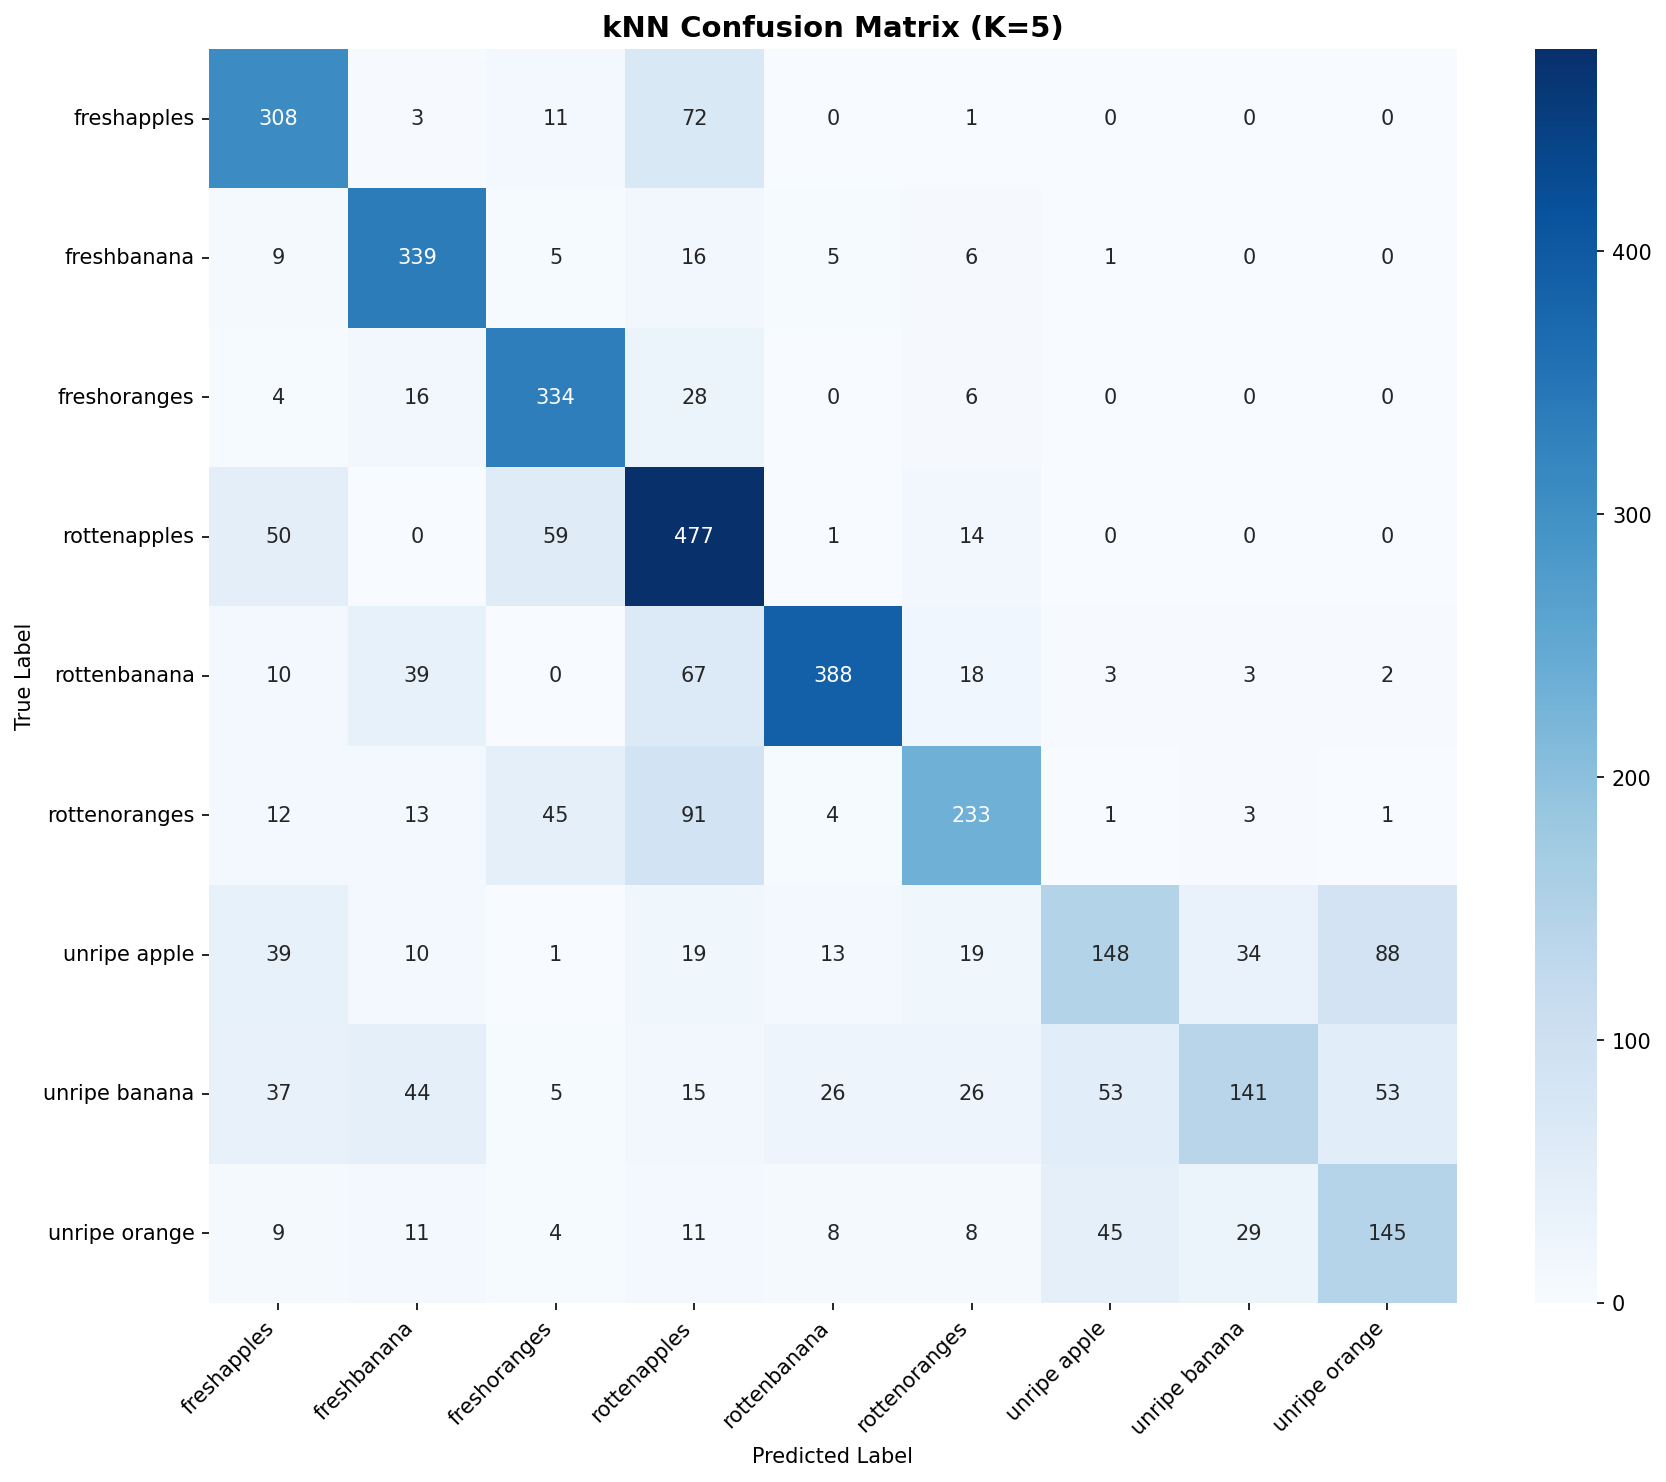
\includegraphics[width=0.7\linewidth]{baseline_knn_confusion_matrix.png}
  \caption{kNN baseline: confusion matrix on test set.}
  \label{fig:knn-conf}
\end{figure}

\begin{figure}[H]
  \centering
  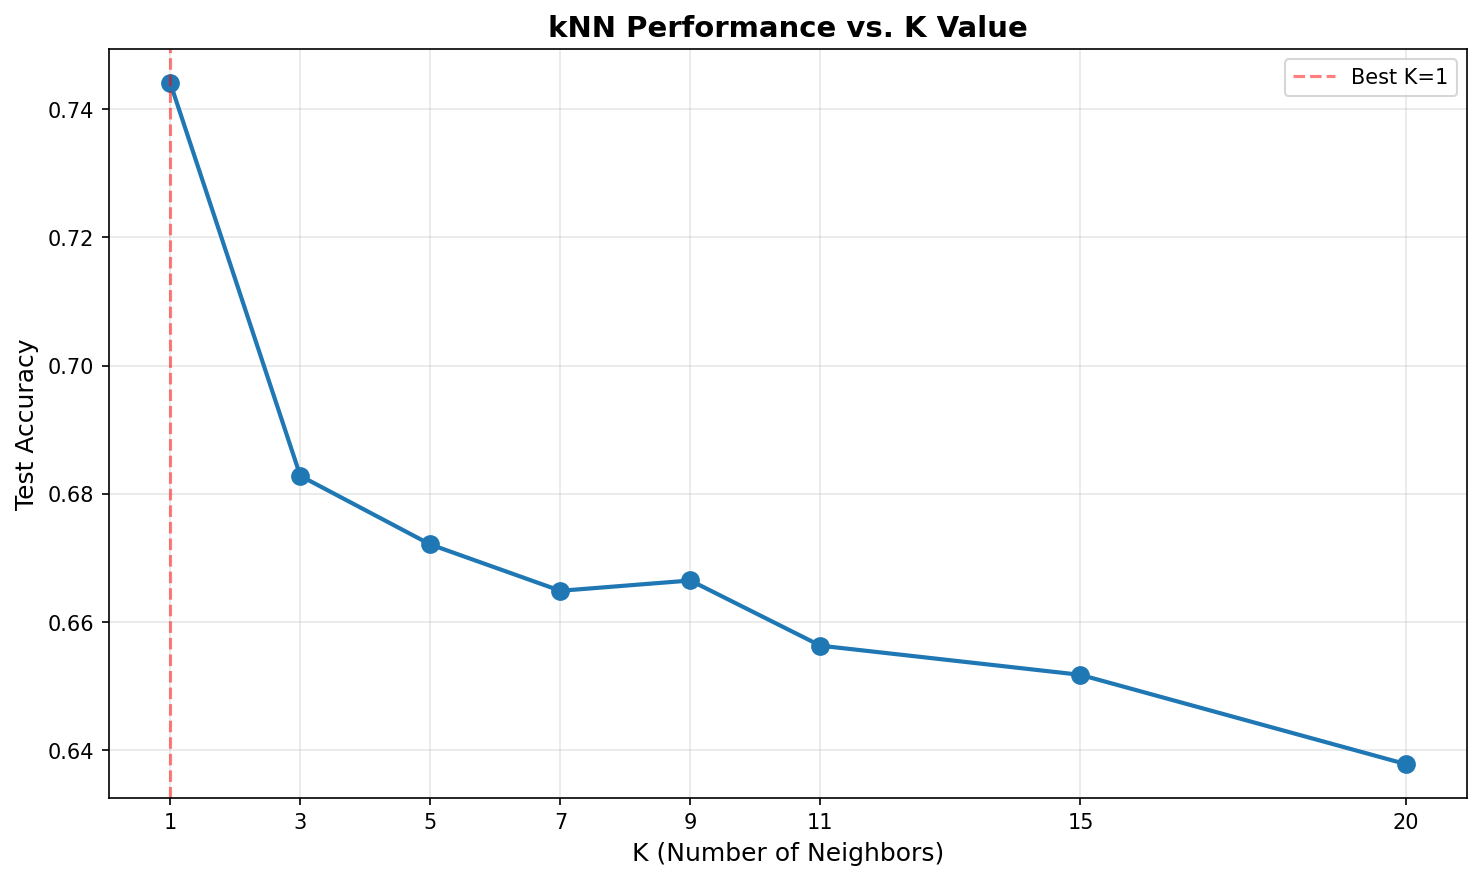
\includegraphics[width=0.6\linewidth]{baseline_knn_k_tuning.png}
  \caption{kNN: effect of K on performance (expected trend).}
  \label{fig:knn-k}
\end{figure}

\subsection{HOG features + Linear Classifiers}
Grayscale images at \(128\times128\) are converted to HOG features and classified with Logistic Regression or Linear SVM. Expected test accuracy is \textasciitilde60--75\% depending on configuration. This approach is fast and interpretable but discards color, which is crucial for ripeness.

\begin{figure}[H]
  \centering
  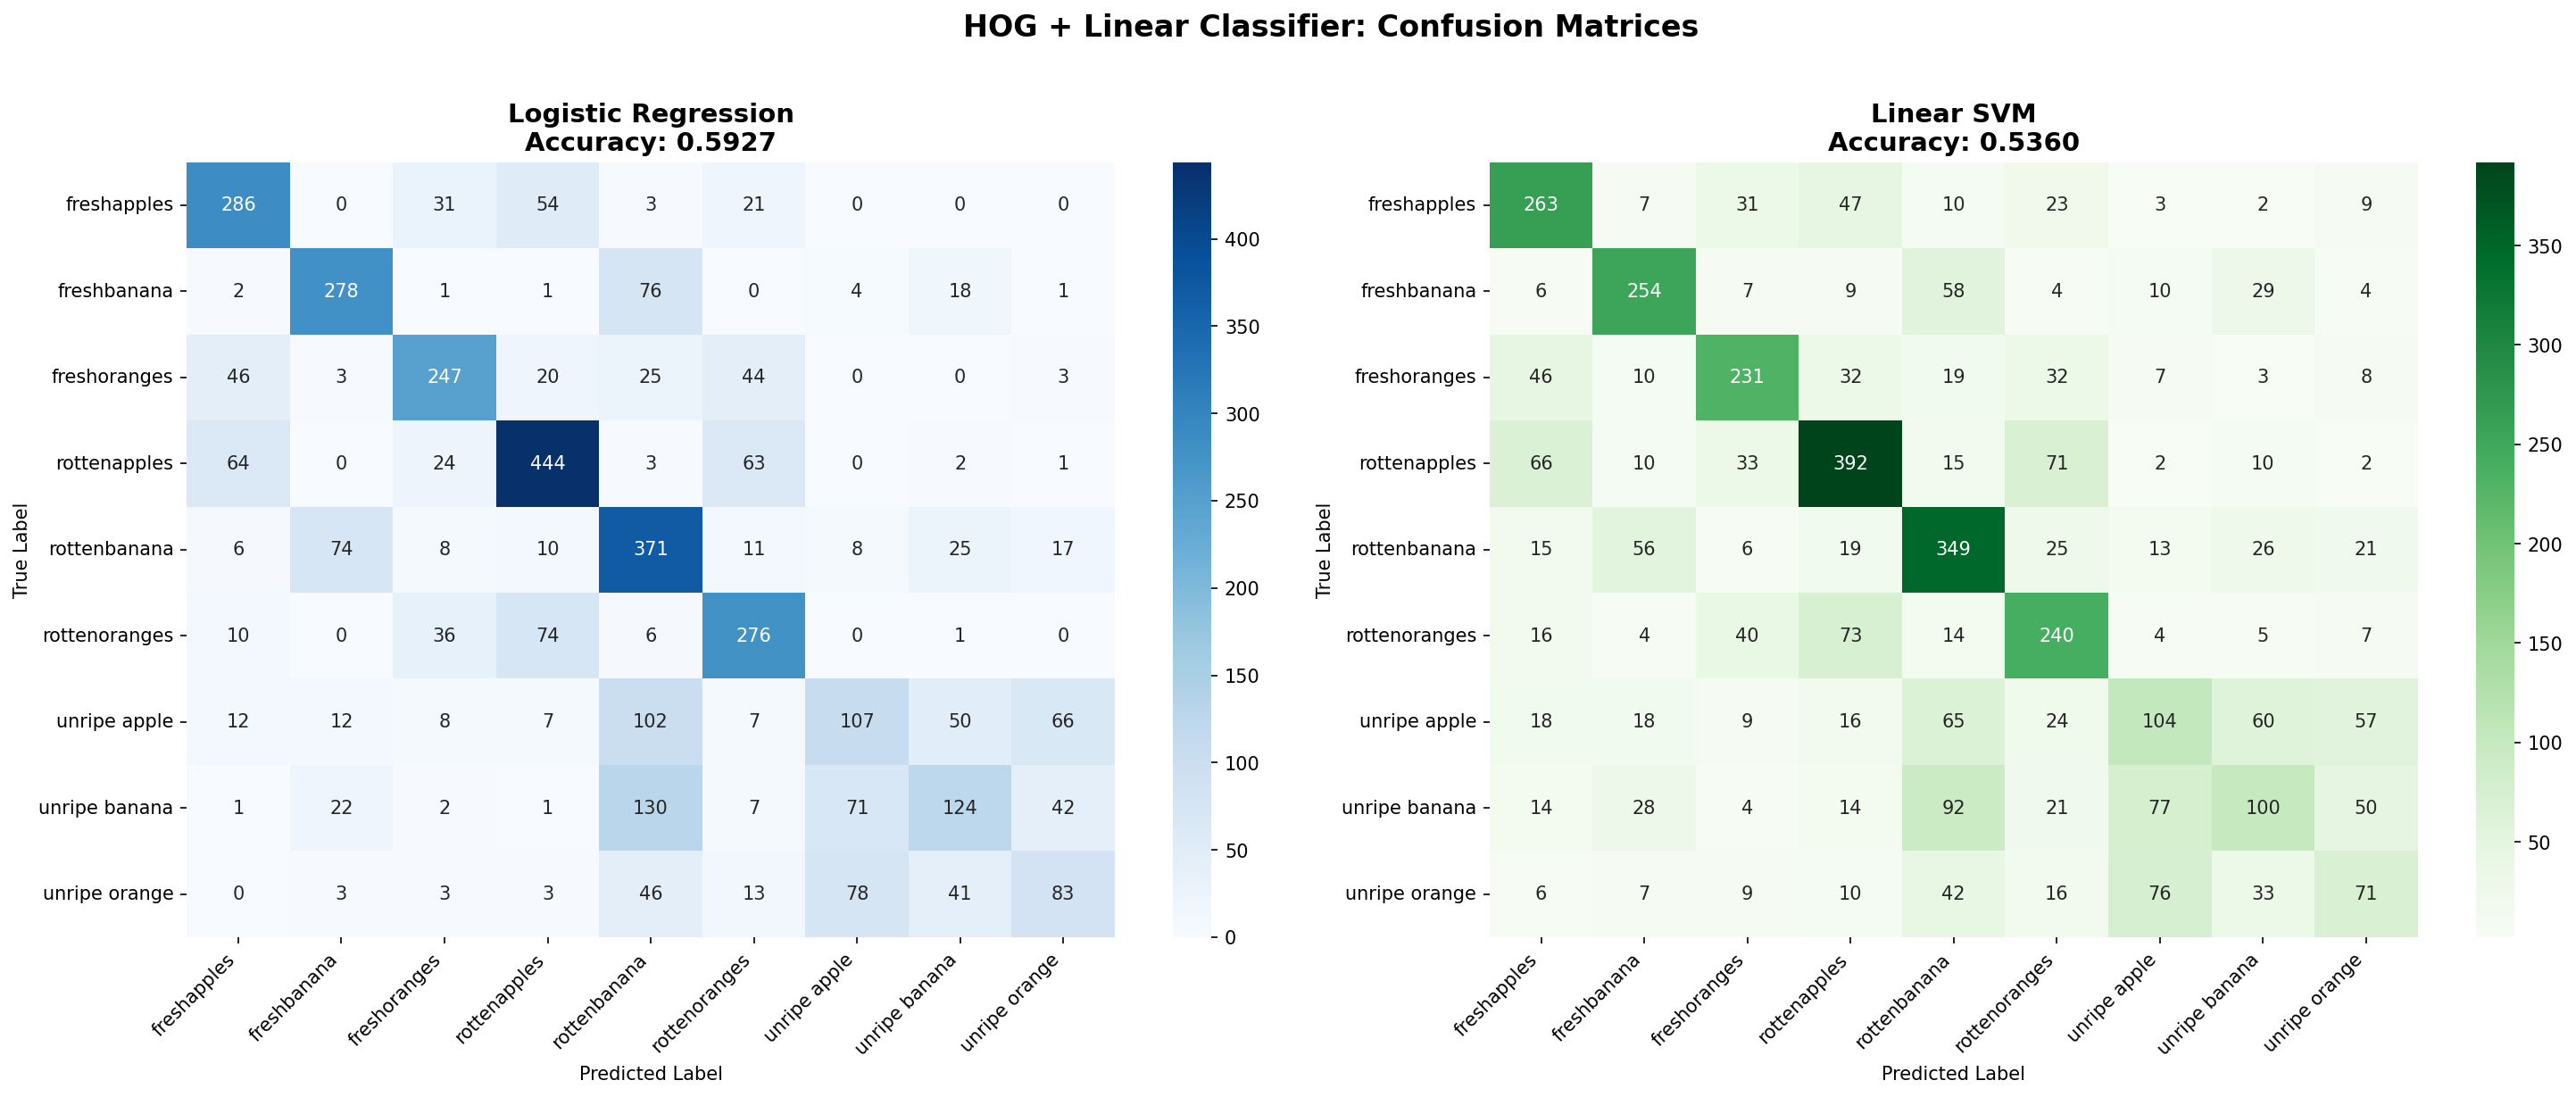
\includegraphics[width=0.75\linewidth]{hog_linear_confusion_matrices.png}
  \caption{HOG + Linear classifiers: confusion matrices (LogReg vs SVM).}
  \label{fig:hog-conf}
\end{figure}

\section{CNN Baseline}
We trained a simple CNN in PyTorch with standard optimisation (cross-entropy loss; AdamW/SGD variants during tuning). Two reference runs are recorded below; final architecture/tuned hyperparameters will follow once sweeps complete.

\subsection{Run 1: 5 epochs}
Seed 42, batch size 32, image size 224, validation split 0.15.\newline
Test loss: 0.678; Test accuracy: \textbf{72.3\%}.

\begin{figure}[H]
  \centering
  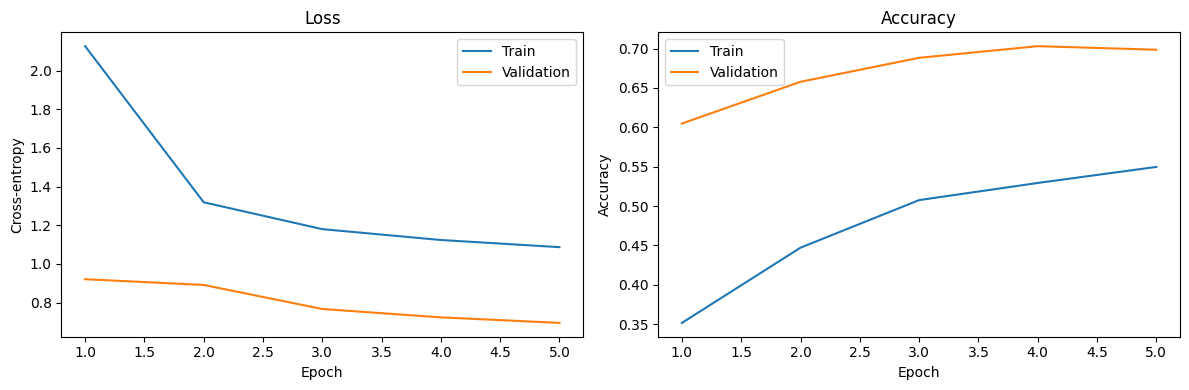
\includegraphics[width=0.85\linewidth]{baseline_cnn_pytorch1.png}
  \caption{CNN training curves (5 epochs).}
  \label{fig:cnn-5ep}
\end{figure}

\subsection{Run 2: 20 epochs}
Same setup, extended training.\newline
Per-epoch metrics show steady improvements in validation accuracy from 0.61 to 0.81.\newline
Final test loss: 0.380; Test accuracy: \textbf{84.5\%}.

\begin{figure}[H]
  \centering
  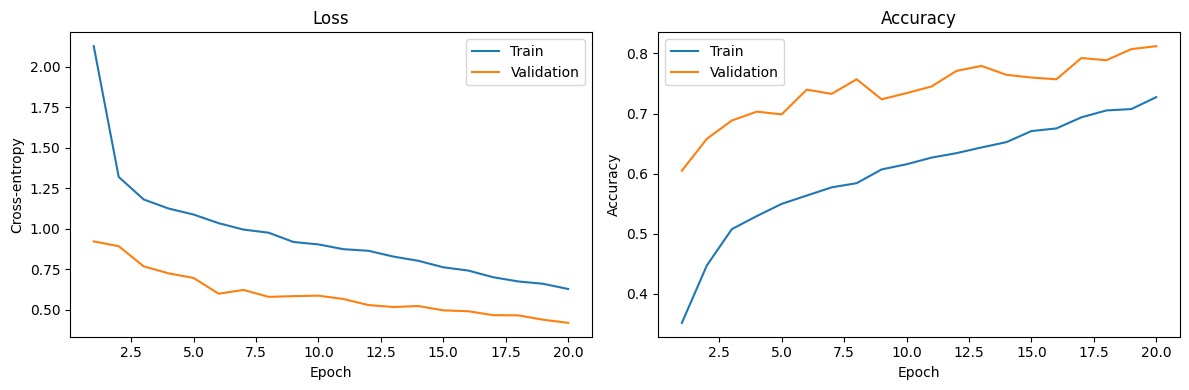
\includegraphics[width=0.85\linewidth]{baseline_cnn_pytorch2.png}
  \caption{CNN training curves (20 epochs).}
  \label{fig:cnn-20ep}
\end{figure}

\section{Hyperparameter Tuning (Methodology)}
Hyperparameter tuning is orchestrated in a Colab-friendly notebook using Weights\,&\,Biases (W\&B) sweeps. The objective maximises validation macro-F1 with early stopping. The search space spans:
\begin{itemize}
  \item Architectures: simple CNN, ResNet-18, MobileNetV3-Small, EfficientNet-B0 (with optional pretrained weights and backbone freezing for ablations).\footnote{Transfer learning is explored methodologically but final submission will adhere to assignment constraints (no fine-tuning of pretrained backbones) unless clarified.}
  \item Optimisers: AdamW/Adam/SGD; scheduler: cosine or ReduceLROnPlateau; label smoothing; gradient clipping.
  \item Data: image size, batch size, augmentation strengths (flip, rotation, color jitter, random erasing).
  \item Regularisation: dropout and weight decay.
\end{itemize}
Results are pending while the tuning runs execute; the best configuration and full metrics table will be inserted here.

\section{Experimental Setup}
\textbf{Frameworks:} PyTorch and torchvision.\newline
\textbf{Environment:} Local and Colab GPU.\newline
\textbf{Reproducibility:} Fixed seeds for data splits and training where applicable; metrics and artefacts logged per run.\newline
\textbf{Evaluation:} Final models are evaluated on the held-out test set; validation drives model selection.

\section{Results Summary}
\begin{center}
\begin{tabular}{lcc}
\toprule
Model & Accuracy & Notes \\
\midrule
Random (9 classes) & 11.1\% & Reference \\
HOG + Linear & 60--75\% & Expected range \\
kNN (raw RGB, K=1) & 74.4\% & Baseline \\
CNN (20 epochs) & 84.5\% & Current best \\
\bottomrule
\end{tabular}
\end{center}
Macro-F1 and per-class metrics will be added alongside CNN confusion matrices.

\section{Analysis}
\textbf{Baselines:} kNN outperforms HOG because color strongly signals ripeness, whereas HOG discards color by design.\newline
\textbf{CNN:} Learns color and texture jointly, outperforming raw-pixel matching by ~10 points. Longer training improves validation and test performance; regularisation and augmentation are expected to further stabilise results.\newline
\textbf{Error patterns:} We expect confusion between adjacent ripeness stages (e.g., ripe vs slightly unripe/rotting). We will quantify this with CNN confusion matrices and a classification report.

\section{Reproducibility}
See \texttt{README.md} for environment setup and dataset download instructions. Notebooks under \texttt{training notebooks/} reproduce baselines and the CNN experiments. Final test predictions and checkpoints will be included in the submission package.

\section{Remaining Work}
We are mid-way through tuning. Outstanding items:\vspace{-0.3em}
\begin{itemize}
  \item Run W\&B sweep; select the best non-pretrained CNN configuration per assignment constraints.
  \item Generate CNN confusion matrix, per-class precision/recall/F1, and classification report.
  \item Add ROC/PR curves (one-vs-rest) for the CNN.
  \item Perform ablations: augmentation on/off, dropout/weight decay sensitivity.
  \item Export final test predictions and save the best checkpoint.
  \item Finalise report sections with tuned results and error analysis.
  \item Prepare 5-minute presentation slides aligned to the marking rubric.
  \item Package submission ZIP with report, code, data sample, and slides.
\end{itemize}

\section*{Acknowledgements}
We acknowledge use of PyTorch, torchvision, scikit-learn, scikit-image, and Weights\,&\,Biases. Baseline methodology and configuration details are documented in the repository under \texttt{training notebooks/}.

\end{document}
